% WINDOWS
% !TEX root = C:\Users\ecos1\Documents\Drone_projects\documentation\witchking_documentation\software\main.tex
\documentclass[11pt]{report}
\usepackage[english]{babel}
\usepackage{natbib}
\usepackage{url}
\usepackage[export]{adjustbox}
\usepackage[utf8x]{inputenc}
\usepackage{mathtools}
\usepackage{graphicx}
\usepackage{titlesec}
\usepackage{listings}
\usepackage{parskip}
\usepackage{fancyhdr}
\usepackage{hyperref}
\usepackage{vmargin}
\usepackage[dvipsnames]{xcolor}
\usepackage[final]{pdfpages}
\usepackage{pdfpages,caption}
\usepackage{footmisc}
\usepackage{float}
\usepackage{subcaption}
\usepackage{multirow}
\usepackage{multicol}
\usepackage{array}
\usepackage{float}
\usepackage{acro}
\usepackage{siunitx}
\newcolumntype{P}[1]{>{\centering\arraybackslash}m{#1}}

%\lstset{language=C,caption={Descriptive Caption Text},label=DescriptiveLabel}
\lstset{ 
  backgroundcolor=\color{white},   % choose the background color; you must add \usepackage{color} or \usepackage{xcolor}; should come as last argument
  basicstyle=\footnotesize,        % the size of the fonts that are used for the code
  breakatwhitespace=false,         % sets if automatic breaks should only happen at whitespace
  breaklines=true,                 % sets automatic line breaking
  captionpos=b,                    % sets the caption-position to bottom
  commentstyle=\color{ForestGreen},    % comment style
  deletekeywords={...},            % if you want to delete keywords from the given language
  escapeinside={\%*}{*)},          % if you want to add LaTeX within your code
  extendedchars=true,              % lets you use non-ASCII characters; for 8-bits encodings only, does not work with UTF-8
  frame=single,	                   % adds a frame around the code
  keepspaces=true,                 % keeps spaces in text, useful for keeping indentation of code (possibly needs columns=flexible)
  keywordstyle=\color{blue},       % keyword style
  language=C,                 % the language of the code
  morekeywords={*,...},            % if you want to add more keywords to the set
  numbers=left,                    % where to put the line-numbers; possible values are (none, left, right)
  numbersep=5pt,                   % how far the line-numbers are from the code
  numberstyle=\tiny\color{gray}, % the style that is used for the line-numbers
  rulecolor=\color{black},         % if not set, the frame-color may be changed on line-breaks within not-black text (e.g. comments (green here))
  showspaces=false,                % show spaces everywhere adding particular underscores; it overrides 'showstringspaces'
  showstringspaces=false,          % underline spaces within strings only
  showtabs=false,                  % show tabs within strings adding particular underscores
  stepnumber=2,                    % the step between two line-numbers. If it's 1, each line will be numbered
  stringstyle=\color{RubineRed},     % string literal style
  tabsize=2,	                   % sets default tabsize to 2 spaces
  title=\lstname                   % show the filename of files included with \lstinputlisting; also try caption instead of title
}
\setboolean{@twoside}{false}
\setmarginsrb{2.5 cm}{2 cm}{2 cm}{2 cm}{2 cm}{1.5 cm}{1 cm}{1.5 cm}
\renewcommand{\baselinestretch}{1.0} 
\titleformat{\chapter}[display]   
{\normalfont\huge\bfseries}{\chaptertitlename\ \thechapter}{20pt}{\Huge}   
\titlespacing*{\chapter}{0pt}{-70pt}{40pt}
\title{\uppercase{\textbf{WitchKing Alpha Manual}}}								% Title
%\author{13103057}								% Author

\pagenumbering{arabic}
\newcolumntype{L}[1]{>{\raggedright\let\newline\\\arraybackslash\hspace{0pt}}m{#1}}
\newcolumntype{C}[1]{>{\centering\let\newline\\\arraybackslash\hspace{0pt}}m{#1}}
\newcolumntype{R}[1]{>{\raggedleft\let\newline\\\arraybackslash\hspace{0pt}}m{#1}}				\let\svthefootnote\thefootnote							

\makeatletter
\let\thetitle\@title
\let\theauthor\@author
\let\thedate\@date
\makeatother

%\pagestyle{fancy}
\fancyhf{}
%\rhead{\theauthor}
%\lhead{\thetitle}
\cfoot{\thepage}

\begin{document}

%%%%%%%%%%%%%%%%%%%%%%%%%%%%%%%%%%%%%%%%%%%%%%%%%%%%%%%%%%%%%%%%%%%%%%%%%%%%%%%%%%%%%%%%%

\begin{titlepage}
	\centering
    \vspace*{0.5 cm}
    
\includegraphics[scale = 0.5]{figures/witch_king_logo.jpg}
				% Course Code
	%\rule{\linewidth}{0.2 mm} \\[1 cm]
	{\Large \bfseries \thetitle}\\
	%\rule{\linewidth}{0.2 mm} \\[1.5 cm]
	\centering
	\vspace{2cm}
    \text{Version: 0.1}\\
    \text{Date: \today}\\
    \text{Initials: Edvardas Vysniauskas}
	
	
    
    
    
    
	
\end{titlepage}

\chapter{Introduction}


\chapter{OS Upgrade}
The Jetpack for Jetson Nano comes with Ubuntu 18.04. There are no official way of upgrading it, however, the community has created a few guides how to make this work. The following guide is made based on \cite{ubuntu_upgrade}.
\section{Install Jetpack}
First, we need to install the latest available JetPack 4.6(L4T 32.6.1). This is the latest downloadable version. However, this will not be the final version before the upgrade. To download the JetPack, use either official source (\url{https://developer.nvidia.com/embedded/jetpack-sdk-46}) or from OneDrive. Use Balena Etcher to flash the image onto the SD card that you will use for the Jetson Nano. Once done, boot the Jetson Nano with the flashed SD card.
\\
Once logged in, perform the usual \textit{sudo apt update} and \textit{sudo apt upgrade}. Once finished, you should have the latest R32.7.6 JetPack. 
This is required to perform the upgrade of the OS, and especially if booting from external drive is required (see \url{https://jetsonhacks.com/2021/03/10/jetson-nano-boot-from-usb/}).
\section{Upgrading from Ubuntu 18.04 to Ubuntu 20.04}
Once you finish upgrading minor version of the JetPack, perform the OS upgrade.
\begin{itemize}
    \item Remove Chromium browser and autoremove redundant packages
    \item Allow release upgrades
    \item Upgrade to Ubuntu 20.04
    \item GCC changes
\end{itemize}
\subsection{Remove Chromium browser and autoremove redundant packages}
The upgrade requires for the Chromium browser to be removed. This is mainly due to Snap installs that will be performed later and the browser can interfere with them (and firefox comes with the upgrade, therefore in the worst case, it is still possible to use the internet browser). To do this, run \textit{sudo apt-get remove --purge chromium-browser chromium-browser-l10n} command. Once it is complete run the following commands:
\begin{lstlisting}[language=bash, belowskip=-0.8 \baselineskip]
# refresh your system
sudo apt-get update
# need nano for editing some files
sudo apt-get install nano
sudo apt-get upgrade
sudo apt-get autoremove
\end{lstlisting}
Next, enable distribution upgrades by setting prompt=normal in the /etc/update-manager/release-upgrades file.
\begin{figure}[h]
    \centering
    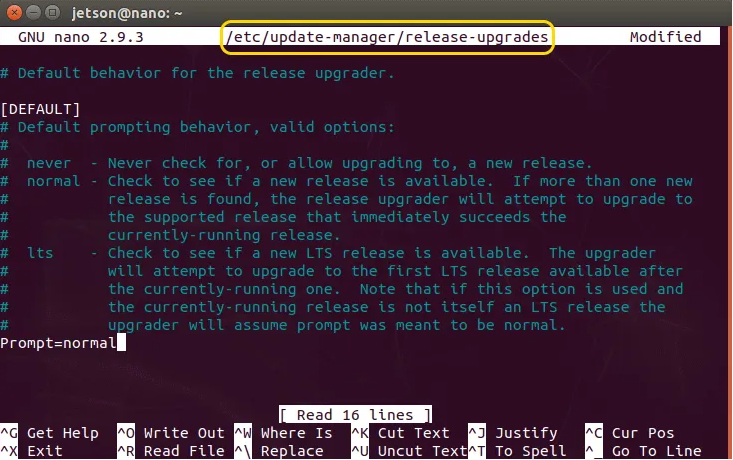
\includegraphics[width=\textwidth]{figures/os_upgrades/distribution_upgrades.PNG}
    \caption{Enable release upgrades.}
    \label{dist_upgrade}
\end{figure}
Again perform regular update-upgrade commands:
\begin{lstlisting}[language=bash, belowskip=-0.8 \baselineskip]
# refresh your system again
sudo apt-get update
sudo apt-get dist-upgrade
sudo reboot
\end{lstlisting}
\subsection{Upgrade to Ubuntu 20.04}
To perform the actual upgrade run \textit{sudo do-release-upgrade} command. This process will take a while, and some prompts will require user input.
Always take the default value, as in some cases the upgrade can become unstable once it is finished (depending on the selection). Once it is finished
it will ask to reboot, but \textbf{do not perform the reboot!!!}
\begin{figure}[h]
    \centering
    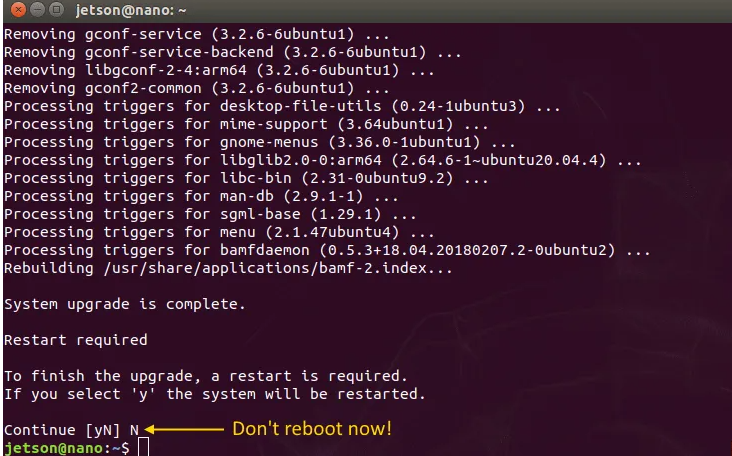
\includegraphics[width=\textwidth]{figures/os_upgrades/do_not_reboot.PNG}
    \caption{Final screen. Do not reboot!}
\end{figure}
Before the reboot, we need to make changes to a few files. Firstly, check that WaylandEnable=false is uncommented in the /etc/gdm3/custom.conf file. Next, uncomment \textit{Driver "nividia"} in the file /etc/X11/xorg.conf. Finally, reverse the dist upgrade setting in the \ref{dist_upgrade} by setting Prompt to \textit{never}. Once done, you can reboot the system.
Once the system boots, remove certain directories that can cause problems. Firstly, delete the /usr/share/vulkan/icd.d directory:
\begin{lstlisting}[language=bash, belowskip=-0.8 \baselineskip]
# remove icd.d
sudo rm -rf /usr/share/vulkan/icd.d
\end{lstlisting}
Then remove other redundant symbolink links in /usr/share/applications and other annoyances:
\begin{lstlisting}[language=bash, belowskip=-0.8 \baselineskip]
# prepare your system
sudo apt-get update
sudo apt-get upgrade
sudo apt-get autoremove
# remove circular symlink
sudo rm /usr/share/applications/vpi1_demos
# remove distorted nvidia logo in top bar
cd /usr/share/nvpmodel_indicator
sudo mv nv_logo.svg no_logo.svg
\end{lstlisting}
Lastly, re-enable the original NVIDIA repositories in /etc/apt/sources.list.d directory. Do the following change to the all existing (should be five) files.
\begin{figure}[h]
    \centering
    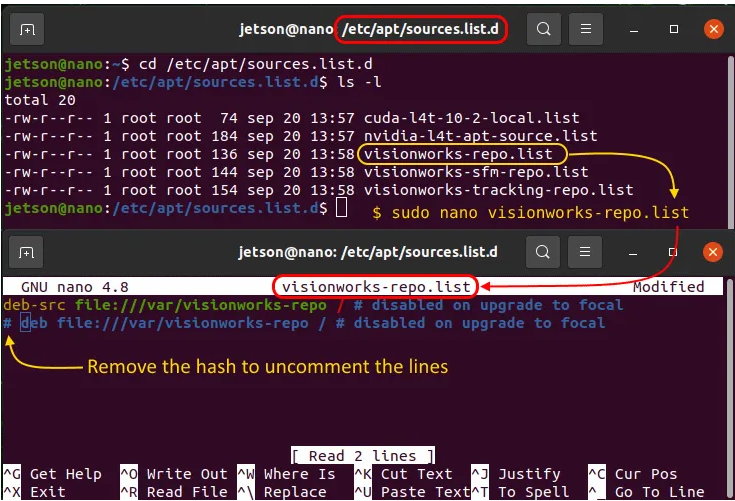
\includegraphics[width=\textwidth]{figures/os_upgrades/nvidia_repositories.PNG}
    \caption{Reactivate NVIDIA repositories.}
\end{figure}
\subsection{GCC changes}
Ubuntu 20.04 comes with GCC 9, but some CUDA packages require GCC 8. To do this, make the following changes to enable both of the versions (perform the same for the clang8):
\begin{lstlisting}[language=bash, belowskip=-0.8 \baselineskip]
# install gcc and g++ version 8
sudo apt-get install gcc-8 g++-8
# setup the gcc selector
sudo update-alternatives --install /usr/bin/gcc gcc /usr/bin/gcc-9 9
sudo update-alternatives --install /usr/bin/gcc gcc /usr/bin/gcc-8 8
# setup the g++ selector
sudo update-alternatives --install /usr/bin/g++ g++ /usr/bin/g++-9 9
sudo update-alternatives --install /usr/bin/g++ g++ /usr/bin/g++-8 8
# if you want to make a selection use these commands
sudo update-alternatives --config gcc
sudo update-alternatives --config g++
\end{lstlisting}
\subsection{Troubleshooting}
It may come a time when you fail to upgrade the existing packages. The problem is the wrong version of the nvidia-l4t-init file. The command \textit{sudo apt --fix-broken install} gives you the following information. In this case, /etc/systemd/sleep.conf is blocking the upgrade. The easiest solution is to force the upgrade with the command \textit{sudo dpkg -i --force-overwrite}. Once done, the upgrade option will work as expected.
\begin{figure}[h]
    \centering
    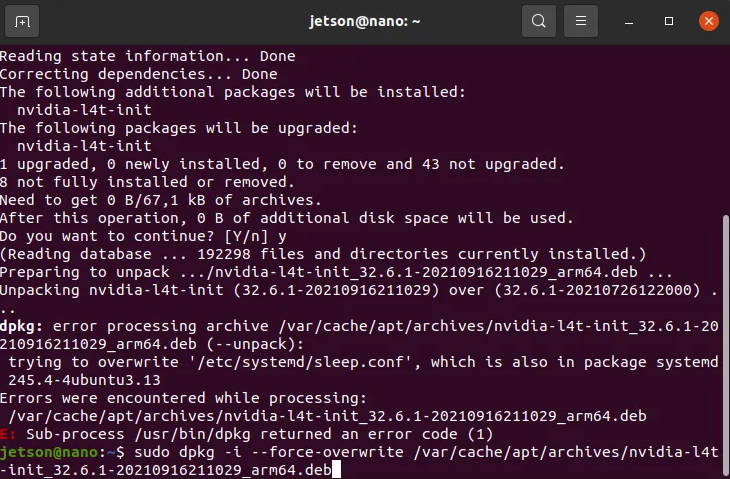
\includegraphics[width=\textwidth]{figures/os_upgrades/fix_broken.PNG}
    \caption{Broken apt upgrade screen.}
\end{figure}

\chapter{Camera Calibration}
Camera calibration is a necessity for removing distorsion from the image. Although there are already made tools for calibrating the camera, such as kalibr \cite{kalibr}


\bibliographystyle{plain}
\bibliography{refs.bib}

\end{document}